% Phase-II Presentation -- EcoRouting Engine (Team DSCPP-III-2026-T186)
% Built on the department-supplied Phase-II.tex template.
% Compile with pdfLaTeX. graphicera_logo.png and app_map.png sit in this folder.

\documentclass[aspectratio=169,11pt]{beamer}

% ============================================================
% PACKAGES
% ============================================================
\usepackage{graphicx}
\usepackage{tikz}
\usetikzlibrary{positioning,arrows.meta}
\usepackage{xcolor}
\usepackage{booktabs}
\usepackage{tabularx}
\usepackage{array}
\usepackage{ragged2e}
\usepackage{hyperref}

% ============================================================
% COLORS - SAME AS PHASE-I
% ============================================================
\definecolor{GEUBlue}{RGB}{20,55,105}
\definecolor{GEULightBlue}{RGB}{238,244,251}
\definecolor{GEUGrey}{RGB}{90,90,90}
\definecolor{GEULightGrey}{RGB}{245,246,248}


% colours and helpers shared with the Phase-II report diagrams
\definecolor{DiagFill}{RGB}{238,244,251}
\definecolor{DiagGrey}{RGB}{90,90,90}
\usetikzlibrary{decorations.pathreplacing,calc}
\newcommand{\formula}[1]{%
    \begin{center}
    \colorbox{DiagFill}{\parbox{0.95\linewidth}{\vspace{3pt}#1\vspace{3pt}}}
    \end{center}
}

% ============================================================
% BEAMER SETTINGS
% ============================================================
\usetheme{default}
\setbeamertemplate{navigation symbols}{}
\setbeamertemplate{blocks}[rounded][shadow=false]

\setbeamercolor{normal text}{fg=black,bg=white}
\setbeamercolor{frametitle}{fg=GEUBlue}
\setbeamercolor{structure}{fg=GEUBlue}
\setbeamercolor{block title}{fg=GEUBlue,bg=GEULightBlue}
\setbeamercolor{block body}{fg=black,bg=GEULightBlue}

\setbeamerfont{frametitle}{size=\Large,series=\bfseries}

% ============================================================
% LOGO
% ============================================================
\newcommand{\GEULogo}{graphicera_logo.png}

% ============================================================
% HEADER
% ============================================================
\setbeamertemplate{headline}{%
  \begin{tikzpicture}[remember picture,overlay]
    \node[
        anchor=north east,
        xshift=-0.30cm,
        yshift=-0.12cm
    ] at (current page.north east)
    {\includegraphics[height=0.62cm]{\GEULogo}};
  \end{tikzpicture}
  \vspace{0.72cm}
}

% ============================================================
% FRAME TITLE
% ============================================================
\setbeamertemplate{frametitle}{%
  \vspace{0.03cm}
  \insertframetitle\par
  \vspace{0.04cm}
  \textcolor{GEUBlue}{\rule{\textwidth}{0.9pt}}
  \vspace{0.03cm}
}

% ============================================================
% FOOTER
% ============================================================
\setbeamertemplate{footline}{%
  \leavevmode
  \hbox{%
  \begin{beamercolorbox}[
      wd=.82\paperwidth,
      ht=0.32cm,
      dp=0.10cm,
      leftskip=.3cm
  ]{author in head/foot}
    \tiny Department of Computer Science \& Engineering |
    Graphic Era (Deemed to be University)
  \end{beamercolorbox}%
  \begin{beamercolorbox}[
      wd=.18\paperwidth,
      ht=0.32cm,
      dp=0.10cm,
      rightskip=.3cm
  ]{date in head/foot}
    \hfill\tiny\insertframenumber/\inserttotalframenumber
  \end{beamercolorbox}}
}

% ============================================================
% CUSTOM COMMANDS
% ============================================================
\newcommand{\smallnote}[1]{%
\vspace{0.08cm}
{\scriptsize\color{GEUGrey}#1}
}

\newcommand{\placeholder}[1]{%
\textit{\color{GEUGrey}#1}
}

% ============================================================
% DOCUMENT INFORMATION
% ============================================================
\title{\textbf{Project-Based Learning}\\[2mm]\large Phase-II Evaluation}
\author{\textbf{EcoRouting Engine}\\Team ID: DSCPP-III-2026-T186}

\institute{
Department of Computer Science \& Engineering\\
Graphic Era (Deemed to be University), Dehradun
}

\date{Academic Session 2026--27}

% ============================================================
% DOCUMENT
% ============================================================
\begin{document}

% ============================================================
% SLIDE 1 -- Title
% ============================================================
\begin{frame}[plain]

\begin{tikzpicture}[remember picture,overlay]

\draw[GEUBlue,line width=3pt]
(current page.north west) -- (current page.north east);

\node[
    anchor=north east,
    xshift=-0.45cm,
    yshift=-0.35cm
] at (current page.north east)
{\includegraphics[height=1.0cm]{\GEULogo}};

\node[
    align=center,
    text width=.84\paperwidth
] at ([yshift=.25cm]current page.center)
{
{\color{GEUBlue}
\fontsize{26}{30}\selectfont
\bfseries PROJECT-BASED LEARNING}
\\[3mm]

{\fontsize{18}{22}\selectfont
PHASE-II EVALUATION}
\\[7mm]

{\color{GEUGrey}
\Large\bfseries
EcoRouting Engine: Hazard-Aware Path Optimization\\and Fill-Rate-Adaptive Waste Scheduling}
\\[3mm]

{\color{GEUBlue}
\normalsize Team ID: DSCPP-III-2026-T186}
};

\node[
    align=center,
    anchor=south,
    yshift=.42cm
] at (current page.south)
{
\bfseries
Department of Computer Science \& Engineering\\
Graphic Era (Deemed to be University), Dehradun\\[-1mm]
\scriptsize Academic Session 2026--27
};

\end{tikzpicture}

\end{frame}

% ============================================================
% SLIDE 2 -- Team & Mentor
% ============================================================
\begin{frame}{Team \& Mentor Details}
\small

\begin{columns}[T,totalwidth=\textwidth]

\column{.48\textwidth}

\begin{block}{Team Information}
\begin{tabular}{@{}ll@{}}
\textbf{Team ID:} & DSCPP-III-2026-T186\\
\textbf{Semester:} & 3rd\\
\textbf{Section:} & A / D / H\\
\textbf{Domain:} & Graph Algorithms (C++)
\end{tabular}
\end{block}

\column{.48\textwidth}

\begin{block}{Team Members}
1.\quad Tejas Jain -- 2510011541 (Team Lead)\\[1mm]
2.\quad Apoorv Negi -- 2510011088\\[1mm]
3.\quad Yash Nigam -- 2510010441
\end{block}

\end{columns}

\vspace{2mm}

\begin{block}{Mentor}
Mr.\ Navneet Rajput
\hfill
\textbf{Interactions completed:}
\underline{\hspace{12mm}}
\end{block}

\end{frame}

% ============================================================
% SLIDE 3 -- Phase-I recap
% ============================================================
\begin{frame}{Phase-I Recap \& Feedback Incorporated}
\scriptsize

\begin{block}{Phase-I Status}
In Phase-I we defined the problem statement, planned the system architecture, chose the tech stack,
and picked a modified (zone-constrained) Dijkstra for hazardous waste and a fill-rate formula for scheduling.
All of that is now built and working.
\end{block}

\vspace{2mm}

\begin{columns}[T,totalwidth=\textwidth]

\column{.48\textwidth}

\textbf{\color{GEUBlue}Feedback Received}

\begin{itemize}\itemsep2pt
\item Fill-rate-based scheduling
\item Public-safety-first route planning for hazardous waste
\item En-route pickups
\item Limit on truck capacity and number of trucks
\end{itemize}

\column{.48\textwidth}

\textbf{\color{GEUBlue}Changes Incorporated}

\begin{itemize}\itemsep2pt
\item Home due once capacity / fill rate days pass (1--14); most overdue first
\item Hazard trucks use constrained Dijkstra on industrial and arterial roads only
\item En-route pickup: later stops on the path are emptied on the way, no backtracking
\item Default sim settings: 3 normal + 2 hazard trucks, 1000 kg per truck; overflow waits a day
\end{itemize}

\end{columns}

\end{frame}

% ============================================================
% SLIDE 4 -- Problem & Objectives
% ============================================================
\begin{frame}{Problem Statement \& Finalized Objectives}
\small

\begin{block}{Problem Statement}
Garbage trucks follow fixed routes every day whether or not there is anything to collect.
Every bin is treated as if it fills at the same rate, and hazardous waste is often collected
with ordinary waste on the same residential streets.
\end{block}

\vspace{2mm}

\textbf{\color{GEUBlue}Finalized Objectives}

\begin{enumerate}\itemsep3pt
\item Model the city as a weighted, zone-tagged graph
\item Build shortest-path collection routes for each truck with Dijkstra's algorithm
\item Schedule pickups from each home's fill rate instead of a fixed timetable
\item Send hazardous waste on industrial and arterial roads only, to the right disposal bin
\end{enumerate}

\end{frame}

% ============================================================
% SLIDE 5 -- Architecture
% ============================================================
\begin{frame}{Updated System Architecture / Workflow}
\scriptsize

\vspace{-3mm}
\begin{center}
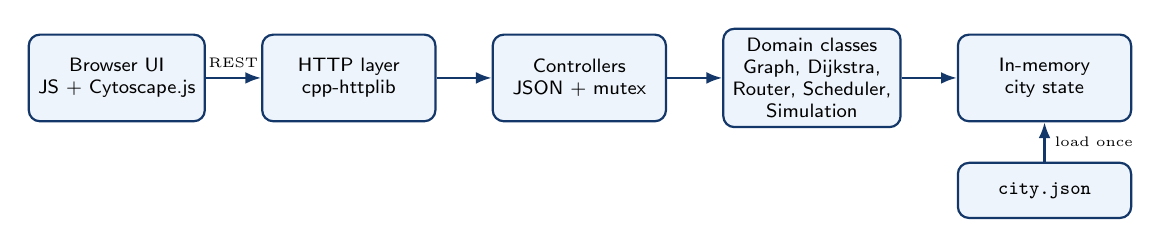
\begin{tikzpicture}[
node distance=7mm,
box/.style={rectangle,rounded corners,draw=GEUBlue,fill=GEULightBlue,thick,minimum width=2.2cm,minimum height=11mm,align=center,font=\scriptsize\sffamily},
arrow/.style={-{Latex[length=2mm]},thick,draw=GEUBlue}
]
\node[box] (a) {Browser UI\\JS + Cytoscape.js};
\node[box,right=of a] (b) {HTTP layer\\cpp-httplib};
\node[box,right=of b] (c) {Controllers\\JSON + mutex};
\node[box,right=of c] (d) {Domain classes\\Graph, Dijkstra,\\Router, Scheduler,\\Simulation};
\node[box,right=of d] (e) {In-memory\\city state};
\node[box,below=5mm of e,minimum height=7mm] (f) {\texttt{city.json}};
\draw[arrow] (a)--node[above,font=\tiny]{REST}(b);
\draw[arrow] (b)--(c); \draw[arrow] (c)--(d); \draw[arrow] (d)--(e);
\draw[arrow] (f)--node[right,font=\tiny]{load once}(e);
\end{tikzpicture}
\end{center}

\vspace{1mm}

\begin{columns}[T,totalwidth=\textwidth]

\column{.48\textwidth}

\textbf{\color{GEUBlue}Major Components}

\begin{itemize}\itemsep1pt
\item One C++17 process serves the API and front end
\item In-memory adjacency-list city from \texttt{city.json}
\item \texttt{RouteStrategy} base; Priority / FIFO subclasses
\item REST + JSON, 13 endpoints, one error format
\end{itemize}

\column{.48\textwidth}

\textbf{\color{GEUBlue}Changes Since Phase-I}

\begin{itemize}\itemsep1pt
\item Day-by-day simulation with a limited fleet
\item En-route pickup in the route builders
\end{itemize}

\end{columns}

\end{frame}

% ============================================================
% SLIDE 5a -- System overview (from the report)
% ============================================================
\begin{frame}{System Overview}
\scriptsize
\setlength{\parskip}{1pt}
\textbf{1.} The clock moves forward one day.

\textbf{2.} A home is due once the days since its last collection reach capacity / fill rate (1--14 days); the most overdue comes first (b).

\textbf{3.} Due bins are emptied, hazardous homes go to the hazard trucks (e), and normal homes are ordered and packed onto trucks before routing (d).

\textbf{4.} Each truck chains shortest paths in its list order:
\formula{\raggedright\ttfamily\tiny
current = DEPOT;\ \ visited = \{ \}\\
for each home in order:\\
\hspace*{4mm}skip it if in visited\\
\hspace*{4mm}path = Dijkstra(current $\to$ home);\ \ if none, mark unreachable\\
\hspace*{4mm}empty later stops on the path, add them to visited\hfill\textrm{\tiny(en-route pickup, (c))}\\
\hspace*{4mm}empty home, add to visited;\ \ current = home\\
then visit the nearest bin for each waste type collected}

\textbf{5.} Served homes get ``last collected = today''; unreachable ones are reported as failed, and carried-over homes rank higher tomorrow.
\end{frame}

% ============================================================
\begin{frame}{Graph Storage, Dijkstra \& Fill-Rate Scheduling}
\begin{center}
{\color{GEUBlue}\bfseries\large (a) Graph Storage and Dijkstra}\\[1mm]
\resizebox{.62\textwidth}{!}{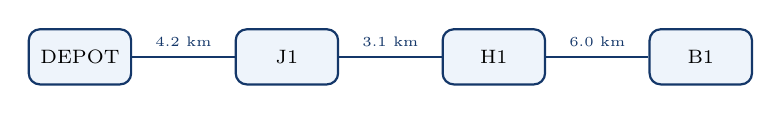
\begin{tikzpicture}[
node distance=13mm,
nd/.style={draw=GEUBlue,fill=DiagFill,thick,rounded corners,minimum width=1.3cm,minimum height=7mm,font=\scriptsize,align=center},
lbl/.style={font=\tiny,draw=none,fill=none}
]
\node[nd] (depot) {DEPOT};
\node[nd,right=of depot] (j1) {J1};
\node[nd,right=of j1] (h1) {H1};
\node[nd,right=of h1] (b1) {B1};
\draw[thick,GEUBlue] (depot)--(j1) node[midway,above,lbl]{4.2 km};
\draw[thick,GEUBlue] (j1)--(h1) node[midway,above,lbl]{3.1 km};
\draw[thick,GEUBlue] (h1)--(b1) node[midway,above,lbl]{6.0 km};
\end{tikzpicture}}\\[2mm]
\resizebox{.55\textwidth}{!}{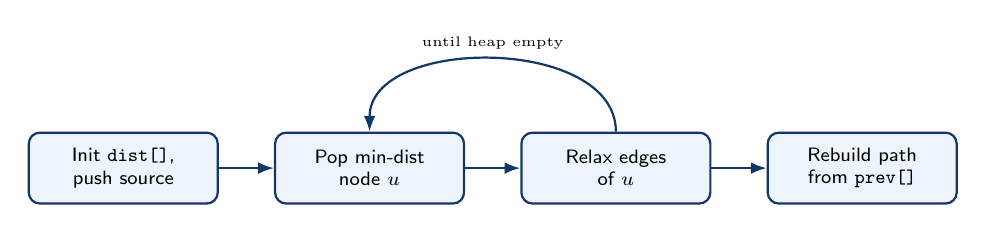
\begin{tikzpicture}[
node distance=7mm,
box/.style={rectangle,rounded corners,draw=GEUBlue,fill=DiagFill,thick,minimum width=2.4cm,minimum height=9mm,align=center,font=\scriptsize\sffamily},
arrow/.style={-{Latex[length=2mm]},thick,draw=GEUBlue}
]
\node[box] (a) {Init \texttt{dist[]},\\push source};
\node[box,right=of a] (b) {Pop min-dist\\node $u$};
\node[box,right=of b] (c) {Relax edges\\of $u$};
\node[box,right=of c] (d) {Rebuild path\\from \texttt{prev[]}};
\draw[arrow] (a)--(b); \draw[arrow] (b)--(c); \draw[arrow] (c)--(d);
\draw[arrow] (c.north) to[out=90,in=90] node[midway,above,font=\tiny]{until heap empty} (b.north);
\end{tikzpicture}}\\[1mm]
{\color{GEUBlue}\bfseries\large (b) Fill-Rate Scheduling}\\[1mm]
\resizebox{.8\textwidth}{!}{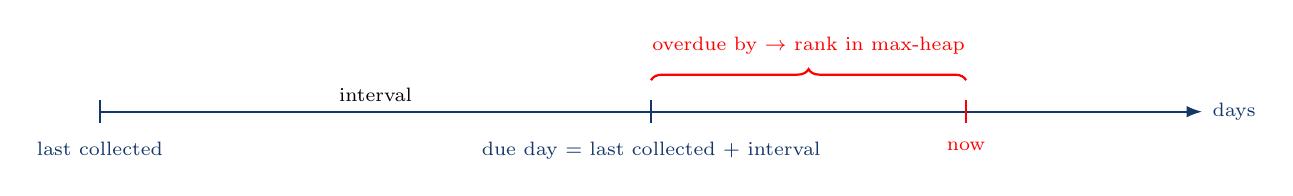
\begin{tikzpicture}[font=\scriptsize]
\draw[thick,GEUBlue,-{Latex[length=2mm]}] (0,0) -- (14,0) node[right]{days};
\draw[thick,GEUBlue] (0,0.15) -- (0,-0.15) node[below,yshift=-1mm]{last collected};
\draw[thick,GEUBlue] (7,0.15) -- (7,-0.15) node[below,yshift=-1mm]{due day = last collected + interval};
\draw[thick,red] (11,0.15) -- (11,-0.15) node[below,yshift=-1mm]{now};
\draw[decorate,decoration={brace,amplitude=4pt},thick,red] (7,0.4) -- (11,0.4) node[midway,above,yshift=2mm]{overdue by $\to$ rank in max-heap};
\node[above] at (3.5,0) {interval};
\end{tikzpicture}}
\end{center}
\end{frame}

% ============================================================
\begin{frame}{(c) En-Route Pickup}
\begin{center}
\resizebox{.95\textwidth}{!}{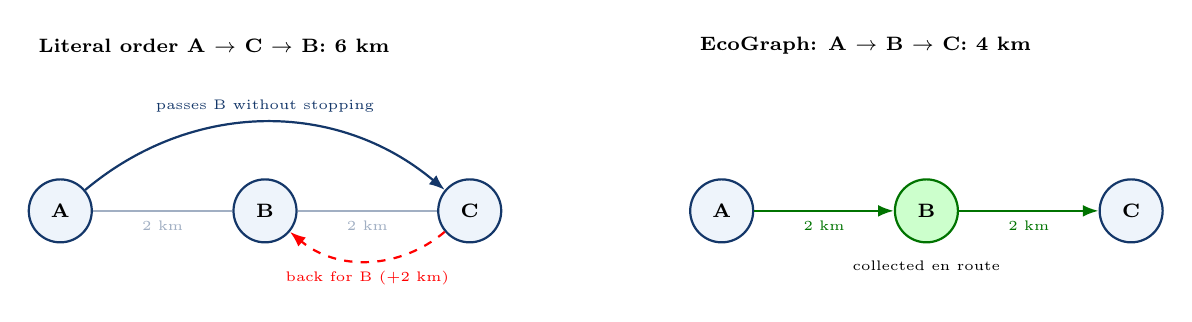
\begin{tikzpicture}[
nd/.style={circle,draw=GEUBlue,fill=DiagFill,thick,minimum size=8mm,font=\scriptsize\bfseries},
lbl/.style={font=\tiny,draw=none,fill=none}
]
% literal order
\node[font=\scriptsize\bfseries,anchor=west] at (-0.4,2.1) {Literal order A $\to$ C $\to$ B: 6 km};
\node[nd] (a1) at (0,0) {A};
\node[nd] (b1) at (2.6,0) {B};
\node[nd] (c1) at (5.2,0) {C};
\draw[thick,GEUBlue!40] (a1)--(b1) node[midway,below,lbl]{2 km};
\draw[thick,GEUBlue!40] (b1)--(c1) node[midway,below,lbl]{2 km};
\draw[-{Latex[length=2mm]},thick,GEUBlue] (a1) to[out=40,in=140] node[midway,above,lbl]{passes B without stopping} (c1);
\draw[-{Latex[length=2mm]},thick,red,dashed] (c1) to[out=-140,in=-40] node[midway,below,lbl]{back for B (+2 km)} (b1);
% en-route
\node[font=\scriptsize\bfseries,anchor=west] at (8.0,2.1) {EcoGraph: A $\to$ B $\to$ C: 4 km};
\node[nd] (a2) at (8.4,0) {A};
\node[nd,fill=green!20,draw=green!45!black] (b2) at (11.0,0) {B};
\node[nd] (c2) at (13.6,0) {C};
\draw[-{Latex[length=2mm]},thick,green!45!black] (a2)--(b2) node[midway,below,lbl]{2 km};
\draw[-{Latex[length=2mm]},thick,green!45!black] (b2)--(c2) node[midway,below,lbl]{2 km};
\node[lbl,below=1mm of b2] {collected en route};
\end{tikzpicture}}
\end{center}
\end{frame}

% ============================================================
\begin{frame}{(d) Truck Fleet and Capacity}
\begin{center}
\resizebox{.95\textwidth}{!}{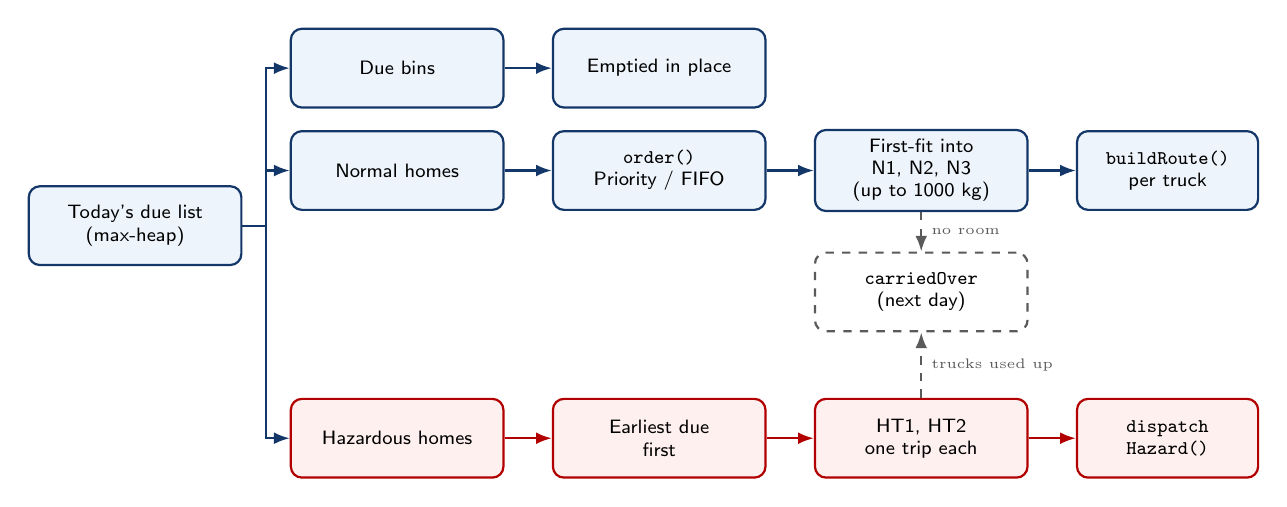
\begin{tikzpicture}[
node distance=5mm and 6mm,
box/.style={rectangle,rounded corners,draw=GEUBlue,fill=DiagFill,thick,minimum width=2.7cm,minimum height=10mm,align=center,font=\scriptsize\sffamily},
hz/.style={box,draw=red!70!black,fill=red!6},
bad/.style={box,draw=DiagGrey,fill=white,dashed},
arrow/.style={-{Latex[length=2mm]},thick,draw=GEUBlue}
]
\node[box,yshift=-7mm] (due) {Today's due list\\(max-heap)};
\node[box,right=of due,yshift=20mm] (bins) {Due bins};
\node[box,right=of due,yshift=7mm] (norm) {Normal homes};
\node[hz,right=of due,yshift=-27mm] (haz) {Hazardous homes};
\node[box,right=of bins] (emp) {Emptied in place};
\node[box,right=of norm] (ord) {\texttt{order()}\\Priority / FIFO};
\node[box,right=of ord] (ff) {First-fit into\\N1, N2, N3\\(up to 1000 kg)};
\node[box,right=of ff,minimum width=2.3cm] (rt) {\texttt{buildRoute()}\\per truck};
\node[hz,right=of haz] (fifo) {Earliest due\\first};
\node[hz,right=of fifo] (ht) {HT1, HT2\\one trip each};
\node[hz,right=of ht,minimum width=2.3cm] (dh) {\texttt{dispatch}\\\texttt{Hazard()}};
\node[bad,below=5mm of ff] (co) {\texttt{carriedOver}\\(next day)};
\draw[arrow] (due.east)--++(3mm,0)|-(bins.west);
\draw[arrow] (due.east)--++(3mm,0)|-(norm.west);
\draw[arrow] (due.east)--++(3mm,0)|-(haz.west);
\draw[arrow] (bins)--(emp); \draw[arrow] (norm)--(ord); \draw[arrow] (ord)--(ff); \draw[arrow] (ff)--(rt);
\draw[arrow,red!70!black] (haz)--(fifo); \draw[arrow,red!70!black] (fifo)--(ht); \draw[arrow,red!70!black] (ht)--(dh);
\draw[arrow,dashed,DiagGrey] (ff)--node[right,font=\tiny]{no room}(co);
\draw[arrow,dashed,DiagGrey] (ht.north)--node[right,font=\tiny]{trucks used up}(co.south);
\end{tikzpicture}}
\end{center}
\end{frame}

% ============================================================
\begin{frame}{(e) Hazard Dispatch \& Constrained Dijkstra}
\begin{center}
\resizebox{.95\textwidth}{!}{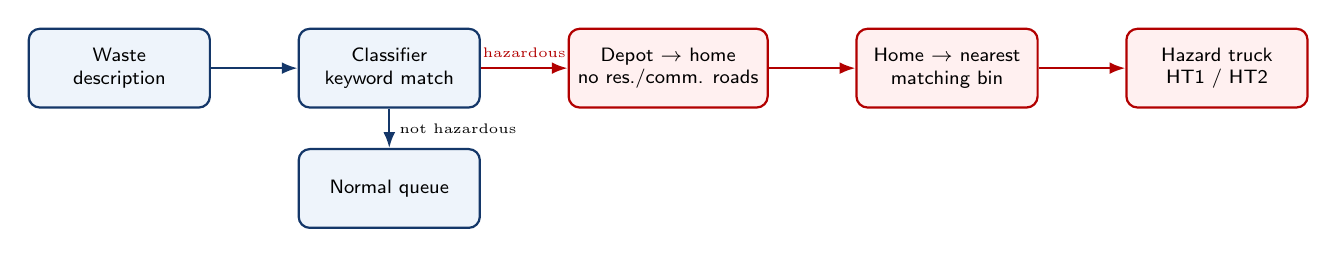
\begin{tikzpicture}[
node distance=11mm,
box/.style={rectangle,rounded corners,draw=GEUBlue,fill=DiagFill,thick,minimum width=2.3cm,minimum height=10mm,align=center,font=\scriptsize\sffamily},
hz/.style={box,draw=red!70!black,fill=red!6},
arrow/.style={-{Latex[length=2mm]},thick,draw=GEUBlue}
]
\node[box] (w) {Waste\\description};
\node[box,right=of w] (cl) {Classifier\\keyword match};
\node[hz,right=of cl] (d1) {Depot $\to$ home\\no res./comm. roads};
\node[hz,right=of d1] (d2) {Home $\to$ nearest\\matching bin};
\node[hz,right=of d2] (tr) {Hazard truck\\HT1 / HT2};
\node[box,below=5mm of cl] (nq) {Normal queue};
\draw[arrow] (w)--(cl);
\draw[arrow,red!70!black] (cl)--node[above,font=\tiny]{hazardous}(d1);
\draw[arrow,red!70!black] (d1)--(d2); \draw[arrow,red!70!black] (d2)--(tr);
\draw[arrow] (cl)--node[right,font=\tiny]{not hazardous}(nq);
\end{tikzpicture}}\\[4mm]
\resizebox{.55\textwidth}{!}{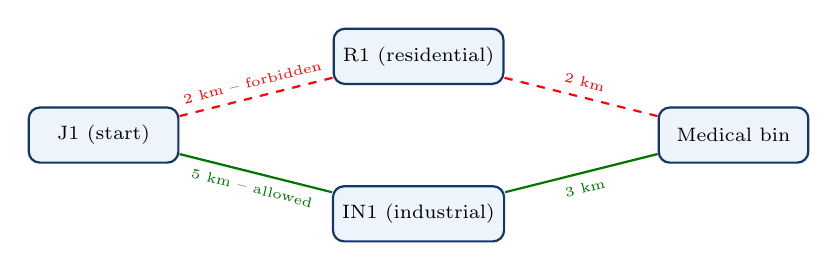
\begin{tikzpicture}[
nd/.style={draw=GEUBlue,fill=DiagFill,thick,rounded corners,minimum width=1.9cm,minimum height=7mm,font=\scriptsize,align=center},
lbl/.style={font=\tiny,draw=none,fill=none}
]
\node[nd] (j1) at (0,0) {J1 (start)};
\node[nd] (r1) at (4,1.0) {R1 (residential)};
\node[nd] (in1) at (4,-1.0) {IN1 (industrial)};
\node[nd] (bin) at (8,0) {Medical bin};
\draw[thick,red,dashed] (j1)--(r1) node[midway,above,sloped,lbl]{2 km -- forbidden};
\draw[thick,red,dashed] (r1)--(bin) node[midway,above,sloped,lbl]{2 km};
\draw[thick,green!45!black] (j1)--(in1) node[midway,below,sloped,lbl]{5 km -- allowed};
\draw[thick,green!45!black] (in1)--(bin) node[midway,below,sloped,lbl]{3 km};
\end{tikzpicture}}
\end{center}
\end{frame}

% ============================================================
\begin{frame}{(f) Simulation Architecture}
\begin{center}
\resizebox{.95\textwidth}{!}{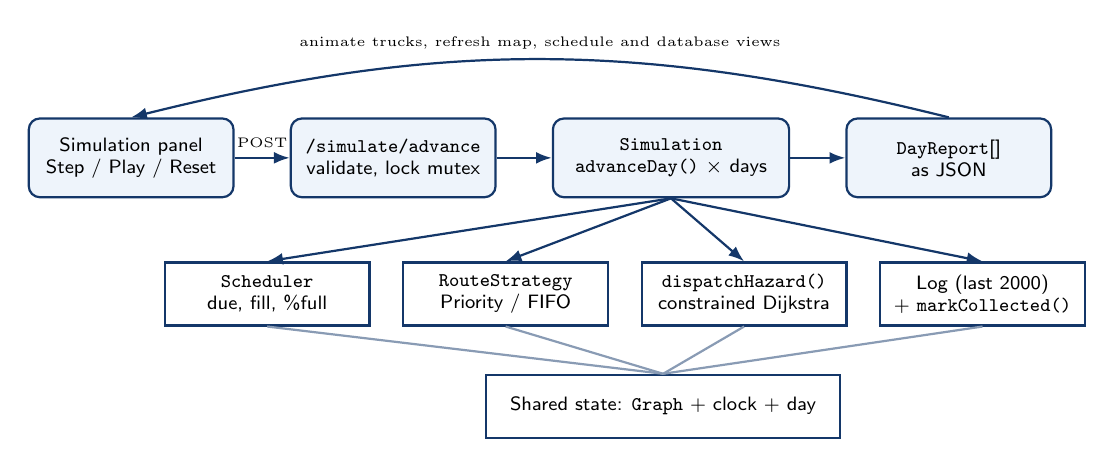
\begin{tikzpicture}[
node distance=6mm and 7mm,
box/.style={rectangle,rounded corners,draw=GEUBlue,fill=DiagFill,thick,minimum width=2.6cm,minimum height=10mm,align=center,font=\scriptsize\sffamily},
st/.style={rectangle,draw=GEUBlue,fill=white,thick,minimum width=2.6cm,minimum height=8mm,align=center,font=\scriptsize\sffamily},
arrow/.style={-{Latex[length=2mm]},thick,draw=GEUBlue}
]
% request path
\node[box] (ui) {Simulation panel\\Step / Play / Reset};
\node[box,right=of ui] (ctl) {\texttt{/simulate/advance}\\validate, lock mutex};
\node[box,right=of ctl,minimum width=3.0cm] (sim) {\texttt{Simulation}\\\texttt{advanceDay()} $\times$ days};
\node[box,right=of sim] (rep) {\texttt{DayReport}[]\\as JSON};
\draw[arrow] (ui)--node[above,font=\tiny]{POST}(ctl);
\draw[arrow] (ctl)--(sim);
\draw[arrow] (sim)--(rep);
\draw[arrow] (rep.north) to[bend right=14] node[above,font=\tiny]{animate trucks, refresh map, schedule and database views} (ui.north);
% collaborators
\node[st,below=8mm of ctl,xshift=-1.6cm] (sch) {\texttt{Scheduler}\\due, fill, \%full};
\node[st,right=4mm of sch] (rs) {\texttt{RouteStrategy}\\Priority / FIFO};
\node[st,right=4mm of rs] (hz) {\texttt{dispatchHazard()}\\constrained Dijkstra};
\node[st,right=4mm of hz] (lg) {Log (last 2000)\\+ \texttt{markCollected()}};
\foreach \n in {sch,rs,hz,lg} \draw[arrow] (sim.south)--(\n.north);
\node[st,below=6mm of rs,xshift=2.0cm,minimum width=4.5cm] (st8) {Shared state: \texttt{Graph} + clock + day};
\foreach \n in {sch,rs,hz,lg} \draw[thick,GEUBlue!50] (\n.south)--(st8.north);
\end{tikzpicture}}
\end{center}
\end{frame}

% ============================================================
% SLIDE 6 -- Modules & requirements
% ============================================================
\begin{frame}{Module Design \& Functional Requirements}
\scriptsize

\begin{columns}[T,totalwidth=\textwidth]

\column{.32\textwidth}

\textbf{\color{GEUBlue}Major Modules}

\begin{enumerate}\itemsep2pt
\item \texttt{graph.cpp}
\item \texttt{dijkstra.cpp}
\item \texttt{scheduler.cpp}
\item \texttt{waste\_classifier.cpp}
\item \texttt{router.cpp}
\item \texttt{simulation.cpp}
\item \texttt{controllers.cpp}
\item \texttt{graph-view.js}
\end{enumerate}

\column{.66\textwidth}

\textbf{\color{GEUBlue}Functional Requirements}

\begin{enumerate}\itemsep2pt
\item City graph as a zone-tagged adjacency list
\item Plain and zone-constrained shortest paths
\item Due, overdue, \% full; max-heap of due homes
\item Classifies waste: medical, chemical, recyclable, compost
\item Priority / FIFO routes, en-route pickup, hazard dispatch
\item Advances days, loads trucks, keeps the collection log
\item 13 REST endpoints as JSON; mutex on shared state
\item Map view and truck route animation
\end{enumerate}

\end{columns}

\vfill

\begin{block}{Module Dependency}
\texttt{simulation.cpp} asks \texttt{scheduler.cpp} what is due; \texttt{router.cpp} builds routes on \texttt{dijkstra.cpp}; \texttt{controllers.cpp} exposes it all.
\end{block}

\end{frame}

% ============================================================
% SLIDE 7 -- Tech stack
% ============================================================
\begin{frame}{Technology Stack \& Development Methodology}
\small

\begin{columns}[T,totalwidth=\textwidth]

\column{.48\textwidth}

\begin{block}{Technology Stack}

\begin{itemize}\itemsep2pt
\item Programming: C++17 (backend), JavaScript (front end)
\item Database: in-memory graph loaded from \texttt{city.json}
\item Framework: cpp-httplib, nlohmann/json, Cytoscape.js
\item Development Tool: GCC 13, CMake / \texttt{build.sh}
\item Version Control: Git / GitHub
\end{itemize}

\end{block}

\column{.48\textwidth}

\begin{block}{Development Methodology}

\begin{enumerate}\itemsep2pt
\item Requirement Analysis
\item System Design
\item Module Development
\item Integration
\item Testing \& Validation
\end{enumerate}

\end{block}

\end{columns}

\end{frame}

% ============================================================
% SLIDE 8 -- Course concepts
% ============================================================
\begin{frame}{Implementation of PBL Course Concepts}
\scriptsize
\begin{center}
\renewcommand{\arraystretch}{1.3}
\begin{tabularx}{.98\textwidth}{@{}>{\bfseries}p{2.6cm}>{\raggedright\arraybackslash}X>{\raggedright\arraybackslash}p{2.7cm}@{}}
\toprule
Course & Concepts Applied & Project Module\\
\midrule
Data Structures in C & Graph (adjacency list), min-heap and max-heap (priority queues), hash map (\texttt{unordered\_map}), path reconstruction via a predecessor map & Graph model, routing engine, scheduler\\
OOPs with C++ & \textbf{Encapsulation} (\texttt{Graph} hides its node/adjacency maps), \textbf{Abstraction} (\texttt{Scheduler} / \texttt{Classifier} expose \texttt{getDueLocations()}, \texttt{classifyWaste()}), \textbf{Inheritance} (\texttt{RouteStrategy} base), \textbf{Polymorphism} (\texttt{PriorityRouteBuilder} / \texttt{FIFORouteBuilder} override virtual \texttt{order()}) & Domain-layer C++ classes\\
\bottomrule
\end{tabularx}
\end{center}
\vfill
\begin{center}
\colorbox{GEULightBlue}{\parbox{.9\textwidth}{\centering
\textbf{Requirement:} The DSA structures come together as a set of C++ classes that put all four OOP pillars to use -- tying Dijkstra, routing and scheduling into one working backend.}}
\end{center}
\end{frame}

% ============================================================
% SLIDE 9 -- Progress
% ============================================================
\begin{frame}{Development \& Implementation Progress}

\scriptsize

\begin{center}

\renewcommand{\arraystretch}{1.25}

\begin{tabularx}{.96\textwidth}
{@{}p{3cm}p{2.2cm}X@{}}

\toprule
\textbf{Module} &
\textbf{Status} &
\textbf{Work Completed}\\
\midrule

Graph + Dijkstra &
Completed &
Zone-tagged adjacency list, plain and constrained Dijkstra\\

Scheduler + Classifier &
Completed &
Fill-rate intervals, due list in a max-heap, keyword waste classifier\\

Router + Hazard Dispatch &
Completed &
Priority / FIFO routes, en-route pickup, hazard trucks on safe roads\\

Simulation + Front End &
Completed &
Day-by-day simulation with limited fleet; map, schedule and database views\\

Deployment &
Pending &
Docker image and hosting\\

\bottomrule

\end{tabularx}

\end{center}

\vspace{1mm}

\begin{center}
\colorbox{GEULightBlue}{
\parbox{.65\textwidth}{
\centering
\textbf{Overall Project Completion:}
80\%
}}
\end{center}

\end{frame}

% ============================================================
% SLIDE 10 -- Prototype
% ============================================================
\begin{frame}{Working Prototype / Demonstration}
\small

\begin{columns}[T,totalwidth=\textwidth]

\column{.45\textwidth}

\textbf{\color{GEUBlue}Implemented Features}

\begin{itemize}\itemsep3pt
\item Dehradun city map with zone-coloured localities
\item Truck routes animated on the map
\item Hazard trucks routed only on industrial and arterial roads
\item Day-by-day simulation with a limited fleet
\end{itemize}

\column{.51\textwidth}

\begin{block}{Prototype / Output}

\centering
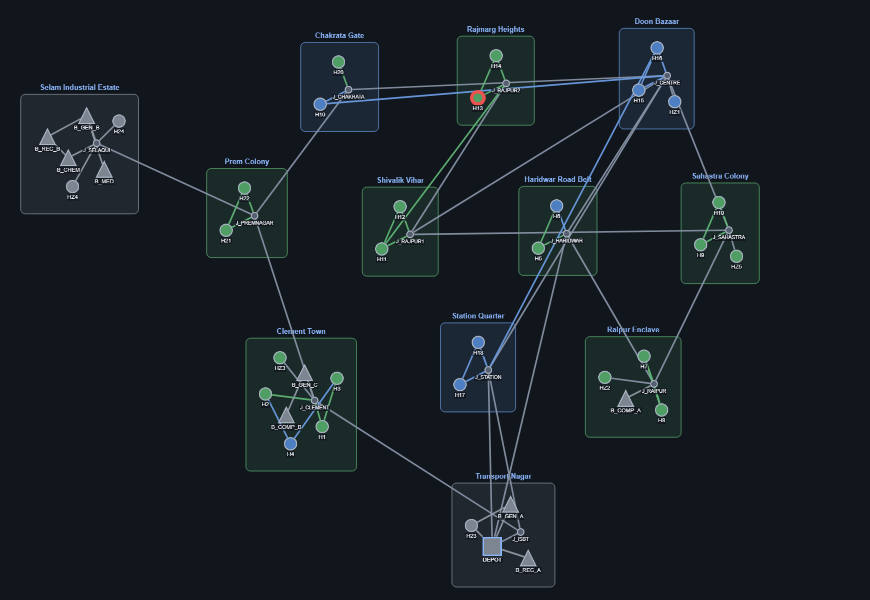
\includegraphics[width=\linewidth,height=4.2cm,keepaspectratio]{app_map.png}

\end{block}

\end{columns}

\end{frame}

% ============================================================
% SLIDE 11 -- Testing
% ============================================================
\begin{frame}{Testing, Results \& Validation}

\scriptsize
\setlength{\parskip}{0pt}

\begin{center}

\renewcommand{\arraystretch}{1.1}

\begin{tabularx}{.96\textwidth}
{@{}p{2.1cm}X X p{1.4cm}@{}}

\toprule
Test / Module &
Expected Result &
Observed Result &
Status\\
\midrule

Dijkstra &
Matches hand-solved graphs; no forbidden road used &
All cases match &
Pass\\

Scheduler / Router &
Intervals in 1--14 days; correct Priority / FIFO order &
All cases match &
Pass\\

Simulation &
Capacity respected; overflow carried to next day &
All cases match &
Pass\\

REST API &
Correct JSON; clean error on bad input &
Checked with curl and the browser &
Pass\\

\bottomrule

\end{tabularx}

\end{center}

\vspace{1mm}

\begin{block}{Results / Validation}
Unit test programs for Dijkstra, the domain classes and the simulation, plus a check of the city data,
all pass. In the A, C, B example, en-route pickup cuts the route from 6 km to 4 km.
\end{block}

\end{frame}

% ============================================================
% SLIDE 12 -- GitHub
% ============================================================
\begin{frame}{GitHub Repository \& Development Activity}
\small

\begin{columns}[T,totalwidth=\textwidth]

\column{.46\textwidth}

\textbf{\color{GEUBlue}Repository Information}

\begin{itemize}\itemsep3pt
\item GitHub Link: \href{https://github.com/Space-Fighter/EcoGraph}{\texttt{github.com/Space-Fighter/EcoGraph}}
\item README.md: Updated, with full API reference
\item Contributors: Tejas Jain, Apoorv Negi
\item Repository Status: Updated
\item Branches: \texttt{main}
\end{itemize}

\column{.50\textwidth}

\textbf{\color{GEUBlue}Development Activity}

\begin{itemize}\itemsep3pt
\item Regular commits maintained
\item Meaningful commit messages
\item Individual contribution visible
\item Latest implementation uploaded
\item Documentation maintained
\end{itemize}

\end{columns}

\end{frame}

% ============================================================
% SLIDE 13 -- Individual contribution
% ============================================================
\begin{frame}{Individual Contribution}

\scriptsize

\begin{center}

\renewcommand{\arraystretch}{1.35}

\begin{tabularx}{.96\textwidth}
{@{}p{2.0cm}>{\raggedright\arraybackslash}p{2.0cm}X p{1.6cm}@{}}

\toprule
Member &
Role &
Technical Contribution &
GitHub Commits\\
\midrule

Tejas Jain &
Team Lead, Backend &
Graph, Dijkstra, scheduler, classifier, route builders, hazard dispatch, simulation, REST server, unit tests &
17\\

Apoorv Negi &
Front End, Docs &
README and API docs, map view, simulation, unit tests, report and presentation &
3\\

Yash Nigam &
Front End &
Schedule, simulation and database views, map view, unit tests, report and presentation &
0\\

\bottomrule

\end{tabularx}

\end{center}

\vspace{3mm}

\begin{block}{Individual Evaluation}
Every member should be prepared to explain and demonstrate
their own technical contribution to the project.
\end{block}

\end{frame}

% ============================================================
% SLIDE 14 -- Challenges & roadmap
% ============================================================
\begin{frame}{Challenges, Remaining Work \& Phase-III Roadmap}
\footnotesize

\begin{columns}[T,totalwidth=\textwidth]

\column{.48\textwidth}

\textbf{\color{GEUBlue}Challenges Faced}

\begin{itemize}\itemsep2pt
\item Hazard truck had no legal roads with only residential / commercial tags
\item Trucks drove past houses on their own list and came back
\item With unlimited trucks, scheduling never showed its effect
\end{itemize}

\vspace{2mm}

\textbf{\color{GEUBlue}Solutions / Learning}

\begin{itemize}\itemsep2pt
\item Added arterial and industrial road classes; en-route pickup
\item Limited fleet (1000 kg per truck) with carry-over to the next day
\end{itemize}

\column{.48\textwidth}

\textbf{\color{GEUBlue}Phase-III Roadmap}

\begin{enumerate}\itemsep3pt
\item Multi-stage Dockerfile for the server and front end
\item Deploy on a container host with auto-redeploy from GitHub
\item Front-end improvements
\item Code cleanup
\item Phase-III report and live demo
\end{enumerate}

\end{columns}

\end{frame}

% ============================================================
% SLIDE 15 -- Outcomes & references
% ============================================================
\begin{frame}{Expected Outcomes \& References}
\small

\begin{columns}[T,totalwidth=\textwidth]

\column{.47\textwidth}

\textbf{\color{GEUBlue}Expected Final Outcomes}

\begin{itemize}\itemsep1pt
\item Working C++ routing and scheduling server with a REST API
\item Shortest-path routes per truck, with en-route pickup
\item Hazardous waste kept off residential and commercial roads
\item Hosted demo reachable from any browser
\end{itemize}

\column{.47\textwidth}

\textbf{\color{GEUBlue}References}

\begin{enumerate}\itemsep0pt
\scriptsize
\item E. W. Dijkstra, ``A Note on Two Problems in Connexion with Graphs,'' 1959
\item Ghiani et al., ``Operations research in solid waste management,'' \textit{Comput.\ Oper.\ Res.}, 2014
\item Cormen et al., \textit{Introduction to Algorithms}, 3rd ed., MIT Press
\item cpp-httplib, nlohmann/json and Cytoscape.js documentation
\end{enumerate}

\vspace{1mm}
\begin{center}

\colorbox{GEUBlue}{
\parbox{.78\textwidth}{
\centering
\color{white}
\textbf{Thank You}\\
Questions \& Suggestions
}}

\end{center}

\end{columns}

\end{frame}

\end{document}
